\documentclass[10pt,letterpaper]{article}

\usepackage[margin=0.95in]{geometry}
\usepackage{amsmath,amssymb,amsfonts}
\usepackage{booktabs}
\usepackage{graphicx}
\usepackage{xcolor}
\usepackage{hyperref}
\usepackage{microtype}
\usepackage{caption}
\usepackage{enumitem}
\usepackage{titlesec}
\usepackage{fancyhdr}

\definecolor{linkblue}{HTML}{1D4ED8}
\hypersetup{
  colorlinks=true,
  linkcolor=linkblue,
  citecolor=linkblue,
  urlcolor=linkblue,
  pdftitle={Looped Hybrid Transformers for Visual SRE Incident Triage},
  pdfauthor={Abhishek Satarkar}
}

\captionsetup{font=small,labelfont=bf}
\setlength{\emergencystretch}{2.5em}
\titleformat{\section}{\large\bfseries}{\thesection.}{0.5em}{}
\titleformat{\subsection}{\normalsize\bfseries}{\thesubsection}{0.5em}{}

\pagestyle{fancy}
\fancyhf{}
\fancyhead[L]{\small\textit{Looped Hybrid Transformers for Visual SRE Incident Triage}}
\fancyhead[R]{\small\textit{A. Satarkar}}
\fancyfoot[C]{\small\thepage}
\renewcommand{\headrulewidth}{0.4pt}

\begin{document}

% ----------------------------------------------------------------------
% arXiv-style Title Block
% ----------------------------------------------------------------------
\begin{center}
\rule{\linewidth}{1.6pt}\\[0.6em]
{\LARGE\bfseries Looped Hybrid Transformers for Visual SRE Incident Triage:\\[0.25em]
\Large Multimodal CoT Distillation, Pure-PyTorch GRPO,\\[0.2em]
and Hybrid-Safe TurboQuant on Consumer Hardware}\\[0.55em]
\rule{\linewidth}{0.8pt}\\[0.9em]
{\large\bfseries Abhishek Satarkar}\\
{\normalsize Independent Researcher}\\
{\small November 2026}
\end{center}
\vspace{0.5em}

% ----------------------------------------------------------------------
% Abstract
% ----------------------------------------------------------------------
\begin{abstract}
\noindent
Small multimodal language models (under 1B parameters) are attractive for local Site Reliability Engineering (SRE) automation, yet stock checkpoints frequently suffer from catastrophic reasoning-loop collapse when tasked with visual telemetry triage and strict JSON tool calling. We present a non-destructive \textbf{Looped Hybrid Transformer} wrapper around \texttt{Qwen/Qwen3.5-0.8B} (18 Gated DeltaNet recurrent layers and 6 Gated Attention layers) trained and evaluated end-to-end on a single consumer 8.00\,GB NVIDIA RTX 4060 Laptop GPU. Our architecture introduces learnable scalar input re-injection after native vision-patch merging, isolated per-loop hybrid KV/recurrent caches (\texttt{PerLoopHybridCache}), and an auxiliary middle-loop cross-entropy objective. On a strictly isolated 15-prompt Visual SRE held-out benchmark featuring dark-mode 2$\times$2 Grafana telemetry dashboards and 5 deterministic operations tools, stock \texttt{Qwen3.5-0.8B} achieves \textbf{0.0\%} tool accuracy with \textbf{100.0\%} \texttt{<think>} truncation. Looped PEFT LoRA SFT distilled from 34 DeepSeek Chain-of-Thought and multi-turn error-recovery traces lifts held-out tool accuracy to \textbf{73.3\%} (0.0\% truncation) while making Loop~2 loss (0.8897) outperform Loop~1 (0.9562). A pure-PyTorch Group Relative Policy Optimization (GRPO) stage using a shared-base frozen reference adapter ($\approx$21\,MB overhead, 3.37\,GB peak VRAM) further raises held-out accuracy to \textbf{86.7\%} (13/15, mean reward $+0.8667$). We additionally evaluate reversible Weight-Space Programming (WSP) directional ablation on MLP \texttt{down\_proj} layers (validating its rollback guardrail once RLVR resolves looping) and introduce \texttt{TurboQuantHybridCache}, which compresses the 6 Gated Attention KV caches by \textbf{4.58$\times$} at 3-bit and \textbf{3.59$\times$} at 4-bit while leaving all 18 Gated DeltaNet states untouched, uncovering an important multimodal visual-patch quantization trade-off.
\end{abstract}

% ----------------------------------------------------------------------
% 1. Introduction
% ----------------------------------------------------------------------
\section{Introduction}
Modern Site Reliability Engineering (SRE) relies heavily on visual telemetry: on-call engineers inspect multi-panel Grafana dashboards (CPU utilization, memory growth, HTTP 5xx error rates, p99 latency, and deployment markers) to distinguish between a bad release requiring a rollback, an organic traffic surge requiring horizontal scaling, a memory-leak OOMKill sawtooth requiring a pod restart, intermittent downstream jitter requiring log inspection, or a multi-service cascading outage requiring immediate escalation. While frontier cloud models can perform multimodal triage, latency, privacy, and cost constraints motivate compact local agents capable of running on a single consumer GPU (8\,GB VRAM).

However, deploying sub-1B reasoning models such as \texttt{Qwen/Qwen3.5-0.8B} \cite{qwen35} on structured multimodal tool calling exposes a severe failure mode: \textit{infinite thinking-loop collapse}. On unseen dark-mode Grafana dashboards, stock \texttt{Qwen3.5-0.8B} enters repetitive internal reasoning inside \texttt{<think>} blocks until hitting the generation limit (100.0\% truncation rate), never closing \texttt{</think>} or emitting valid JSON.

In this work, we investigate whether test-time depth via weight-tied looping \cite{looped}, combined with multimodal Chain-of-Thought (CoT) distillation, pure-PyTorch Reinforcement Learning with Verifiable Rewards (RLVR) \cite{deepseekr1}, surgical weight-space probing \cite{wsp}, and hybrid-aware KV-cache quantization \cite{turboquant}, can turn a 0.8B hybrid model into an accurate Visual SRE triage agent on consumer hardware. Our main contributions are:
\begin{enumerate}[leftmargin=1.5em,itemsep=2pt,topsep=3pt]
    \item \textbf{Looped Hybrid Qwen3.5 Architecture:} A non-destructive PyTorch wrapper adding configurable decoder depth (\texttt{num\_loops}) with post-vision scalar input re-injection and isolated per-loop hybrid caches (\texttt{PerLoopHybridCache}) that preserve Gated DeltaNet recurrence integrity and achieve bit-exact equivalence ($0.000000$ max logit difference) at \texttt{num\_loops=1}.
    \item \textbf{Visual SRE Benchmark \& Leakage-Proof Distillation:} A synthetic dark-mode Grafana benchmark (50 balanced scenarios across 5 deterministic SRE tools, 40 multimodal + 10 text alerts) with SHA-256 verified zero-overlap splits (35 train / 15 held-out) and DeepSeek CoT + 25\% multi-turn error-recovery harvesting.
    \item \textbf{8\,GB Pure-PyTorch SFT \& GRPO Pipeline:} Assistant-only masked LoRA SFT targeting all 12 text-decoder linear projections (10.82M trainable parameters, 1.25\%) followed by pure-PyTorch GRPO using a shared-base frozen reference adapter ($\approx$21\,MB overhead, 3.37\,GB peak VRAM), lifting held-out accuracy from 0.0\% to 73.3\% (SFT) to 86.7\% (GRPO).
    \item \textbf{Surgical WSP Audit \& Hybrid-Safe TurboQuant:} Reversible MLP \texttt{down\_proj} directional ablation with a strict held-out rollback guardrail, plus \texttt{TurboQuantHybridCache} achieving 4.58$\times$ Attention KV compression at 3-bit while revealing a key accuracy-vs-compression trade-off on dense visual patch tokens.
\end{enumerate}

% ----------------------------------------------------------------------
% 2. Architecture
% ----------------------------------------------------------------------
\section{Architecture: Looped Hybrid Qwen3.5}
\subsection{Hybrid Backbone Anatomy}
Inspection of \texttt{transformers==5.24.0} confirms that \texttt{Qwen3\_5ForConditionalGeneration} (\texttt{0.8B}) combines a native patch-merging vision encoder (\texttt{Qwen3\_5VisionModel}) with a 24-layer hybrid text decoder (\texttt{Qwen3\_5TextModel}, hidden size 1024, head dimension $d=256$, 2 KV heads). The 24 layers follow a 3:1 hybrid ratio: \textbf{18 Gated DeltaNet} (\texttt{linear\_attention}) recurrent layers interleaved with \textbf{6 Gated Attention} (\texttt{full\_attention}) layers at indices $\{3, 7, 11, 15, 19, 23\}$. Positional encoding uses 3D Multimodal RoPE (M-RoPE) with 4-row position tensors $[p_{\text{text}}, p_T, p_H, p_W]$ and dual masks (\texttt{create\_causal\_mask} and \texttt{create\_recurrent\_attention\_mask}).

\subsection{Scalar Input Re-Injection for Multimodal Grounding}
Passing hidden states repeatedly through a deep weight-tied stack can cause representation drift away from visual tokens. In \texttt{LoopedQwen3\_5ForConditionalGeneration}, we first execute the native vision encoder once and scatter visual patch embeddings into the token sequence to form $E_{\text{base}} \in \mathbb{R}^{B \times S \times D}$. Letting $\mathcal{F}_\theta$ denote one full pass through all 24 hybrid decoder layers, we initialize $h^{(0)} = E_{\text{base}}$ and apply a learnable fp32 scalar logit $\alpha \in \mathbb{R}$ (initialized to $\alpha_0 = 4.6$, giving $w = \sigma(4.6) \approx 0.99005$) before every loop step $t \ge 1$:
\begin{equation}
    \tilde{h}^{(t)} =
    \begin{cases}
        E_{\text{base}}, & t = 0, \\
        \sigma(\alpha)\, E_{\text{base}} + (1 - \sigma(\alpha))\, h^{(t)}, & t \ge 1,
    \end{cases}
    \qquad
    h^{(t+1)} = \mathcal{F}_\theta\!\left(\tilde{h}^{(t)};\, \mathcal{C}^{(t)}\right),
    \label{eq:loop_reinject}
\end{equation}
for $t \in \{0, \dots, L-1\}$, where $L = \texttt{num\_loops}$. Final logits are produced by applying RMSNorm and \texttt{lm\_head} to $h^{(L)}$. When $L=1$, re-injection is bypassed, guaranteeing bit-exact equivalence with stock \texttt{Qwen3\_5ForConditionalGeneration}.

\subsection{Per-Loop Hybrid Cache Isolation \& Auxiliary Loss}
In \texttt{transformers==5.24.0}, Qwen3.5 stores both Gated Attention KV tensors and Gated DeltaNet causal convolution and recurrent state tensors inside \texttt{DynamicCache(config=text\_config)}. Sharing a single cache across $L$ loops would update each DeltaNet recurrent state $L$ times per decoded token, corrupting the linear recurrence. Our \texttt{PerLoopHybridCache} allocates $L$ independent cache objects $[\mathcal{C}^{(0)}, \dots, \mathcal{C}^{(L-1)}]$ during cached decoding (\texttt{use\_cache=True}), ensuring loop $t$ reads and mutates only $\mathcal{C}^{(t)}$. During training (\texttt{use\_cache=False}), no recurrent state is shared across loops.

To ensure intermediate loop passes receive direct supervision during SFT, we combine the final-loop cross-entropy loss $\mathcal{L}^{(L-1)}$ with an auxiliary middle-loop loss weighted by $\lambda_{\text{aux}} = 0.1$:
\begin{equation}
    \mathcal{L}_{\text{total}} = (1 - \lambda_{\text{aux}})\,\mathcal{L}^{(L-1)} + \frac{\lambda_{\text{aux}}}{L - 1} \sum_{t=0}^{L-2} \mathcal{L}^{(t)}.
    \label{eq:aux_loss}
\end{equation}

% ----------------------------------------------------------------------
% 3. Training & Optimization Pipeline
% ----------------------------------------------------------------------
\section{Training \& Optimization Pipeline}
\subsection{Visual SRE Benchmark \& Leakage-Proof Splits}
We constructed a 50-scenario Visual SRE Incident Triage benchmark (\texttt{generate\_sre\_dataset.py}) balanced across 5 deterministic JSON tool schemas: \texttt{trigger\_rollback}, \texttt{scale\_service}, \texttt{restart\_pod\_pool}, \texttt{query\_logs}, and \texttt{create\_incident} (10 scenarios per tool: 80\% multimodal dark-mode 2$\times$2 Grafana PNG dashboards rendered via \texttt{matplotlib}, 20\% text-only alert logs). Each dashboard encodes distinct visual telemetry signatures (deploy-triggered 5xx cliff, organic RPS/CPU saturation with $<1\%$ errors, 15-minute OOMKill memory sawtooth, intermittent downstream latency jitter, or multi-service cascading SLO breach). Deterministic stratified splitting (\texttt{build\_splits.py}, seed 42) partitions the 50 prompts into \textbf{35 training prompts} (7 per tool) and \textbf{15 strictly held-out evaluation prompts} (3 per tool). A SHA-256 manifest (\texttt{split\_manifest.json}) verifies \textbf{0 overlapping IDs} and \textbf{0 overlapping normalized prompt strings}.

\subsection{DeepSeek CoT Distillation \& Looped LoRA SFT}
Using a non-interactive wrapper around \texttt{opencode run} targeting \texttt{opencode/deepseek-v4.1-flash-free} (with prompts piped over \texttt{stdin} and strict schema rejection sampling), we harvested \textbf{34 validated CoT traces} strictly from the 35 training prompts, including \textbf{8 multi-turn error-recovery traces} (25\% recovery ratio: simulated schema validation error followed by self-correcting \texttt{<think>} and repaired JSON).

For SFT (\texttt{train\_looped\_sft.py}), we froze the vision encoder and base weights, attached PEFT LoRA \cite{lora} ($r=16, \alpha_{\text{lora}}=32, \text{dropout}=0.05$) to all 12 verified text-decoder linear leaf modules (\texttt{q\_proj}, \texttt{k\_proj}, \texttt{v\_proj}, \texttt{o\_proj}, \texttt{in\_proj\_qkv}, \texttt{in\_proj\_z}, \texttt{in\_proj\_b}, \texttt{in\_proj\_a}, \texttt{out\_proj}, \texttt{gate\_proj}, \texttt{up\_proj}, \texttt{down\_proj}; zero overlap with vision linear names), and kept \texttt{reinject\_logit} trainable (10,822,657 trainable parameters, 1.25\% of 863.8M). Training used assistant-only loss masking (masking all system, user, and \texttt{<|im\_start|>assistant\textbackslash n} tokens with $-100$), non-reentrant gradient checkpointing, AdamW ($\text{lr}=2\times10^{-4}$, cosine schedule, \texttt{grad\_accum=4}), and 3 epochs with best-epoch checkpoint selection via held-out \texttt{compare\_loop\_losses(1, 2, 3)}.

\subsection{Pure-PyTorch GRPO (RLVR) on 8\,GB VRAM}
To optimize end-to-end tool execution without TRL wrapper conflicts against \texttt{PerLoopHybridCache}, we implemented GRPO \cite{deepseekr1} directly in PyTorch (\texttt{train\_looped\_grpo.py}). For each training prompt, we sample $G=4$ completions via \texttt{generate\_looped} ($T=0.8$, $p=0.95$, \texttt{max\_new\_tokens=192}) and score each completion deterministically with \texttt{rewards.py}: $+0.15$ for valid \texttt{<think>...</think>} + JSON format, $+0.35$ for full JSON Schema compliance, $+0.50$ for exact \texttt{expected\_tool} match, and a $-0.05$ to $-0.20$ anti-ramble/truncation penalty. Group-relative advantages $A_i = (r_i - \bar{r}) / (\sigma_r + 10^{-6})$ skip updates cleanly whenever $\sigma_r < 10^{-6}$.

To stay well under 8\,GB VRAM, we avoid loading a second 1.62\,GB reference model: instead, we attach a frozen \texttt{ref} copy of the SFT LoRA adapter ($\approx$21\,MB) onto the \textit{same} base weights and swap active adapters under \texttt{torch.no\_grad()} to compute reference log-probabilities $\log \pi_{\text{ref}}$. Policy gradients are micro-batched one rollout at a time using the clipped surrogate objective with Schulman's non-negative KL estimator ($\epsilon=0.2, \beta=0.02, \text{lr}=1\times10^{-5}$):
\begin{equation}
    \mathcal{L}_{\text{GRPO}} = \frac{1}{G} \sum_{i=1}^{G} \left[ -\min\!\left(\rho_i A_i,\, \text{clip}(\rho_i, 1-\epsilon, 1+\epsilon)\,A_i\right) + \beta \left(e^{\Delta_i} - \Delta_i - 1\right) \right],
    \label{eq:grpo}
\end{equation}
where $\rho_i = \exp(\log \pi_\theta - \log \pi_{\text{old}})$ and $\Delta_i = \log \pi_{\text{ref}} - \log \pi_\theta$ are averaged over completion tokens only.

\subsection{Weight-Space Programming (WSP) Guardrail}
Following MIT CSAIL's Weight-Space Programming methodology \cite{wsp}, \texttt{weight\_editor.py} hooks all 24 MLP \texttt{down\_proj} outputs on held-out passing vs. failing traces, computes the contrastive bug direction $d_{\ell} = \mu_{\text{fail},\ell} - \mu_{\text{pass},\ell}$, selects the top 2 layers by $\|d_\ell\|_2$ and top 64 contributing columns ($131{,}072$ weights = $0.0152\%$ of total parameters), and sweeps reversible directional ablation $W_{:,c} \leftarrow W_{:,c} - \alpha\,(\hat{d}_\ell^\top W_{:,c})\,\hat{d}_\ell$ over $\alpha \in \{0.10, 0.25\}$. A strict rollback guardrail commits the patch only if held-out Mean Reward or Tool Accuracy strictly improves without increasing truncation or failure count.

\subsection{Hybrid-Safe TurboQuant KV Compression}
Our \texttt{TurboQuantHybridCache} subclasses \texttt{DynamicCache} and replaces only the 6 \texttt{full\_attention} \texttt{DynamicLayer} slots with \texttt{TurboQuantLayer} (retaining a recent \texttt{bf16} buffer of \texttt{residual\_window=64} tokens), leaving all 18 \texttt{LinearAttentionLayer} DeltaNet states untouched in native \texttt{bf16}/\texttt{fp32}. For each flushed KV vector $x \in \mathbb{R}^d$ ($d=256$), we store its fp16 norm $\|x\|_2$, rotate via a fixed Haar-orthogonal matrix $R$ ($x_{\text{rot}} = (x / \|x\|_2) R$), and quantize using symmetric Gaussian Lloyd-Max centroids scaled by $1/\sqrt{d}$ bit-packed into \texttt{torch.uint8} (2-bit for 3-bit keys, 3-bit for 3-bit values). For keys, Stage~2 projects the residual $e = x_{\text{rot}} - \hat{x}_{\text{rot}}$ through a fixed Gaussian matrix $P$, packing 1-bit signs into \texttt{uint8} (8 signs/byte) and reconstructing unbiased inner products via $\hat{e} = \frac{\sqrt{\pi/2}}{d}\|e\|_2 (s P^\top)$.

% ----------------------------------------------------------------------
% 4. Experimental Results
% ----------------------------------------------------------------------
\section{Experimental Results \& Ablation Study}
All experiments were executed on a single NVIDIA GeForce RTX 4060 Laptop GPU (8.00\,GB VRAM) in \texttt{bfloat16} using \texttt{torch==2.11.0+cu128}, \texttt{transformers==5.24.0}, and \texttt{peft==0.22.0}. Table~\ref{tab:ablation} reports the complete held-out evaluation progression across all 15 unseen Visual SRE prompts, and Table~\ref{tab:turboquant} details the long-context TurboQuant KV-cache benchmark at 2064 tokens (\texttt{num\_loops=2}).

\begin{figure}[t]
    \centering
    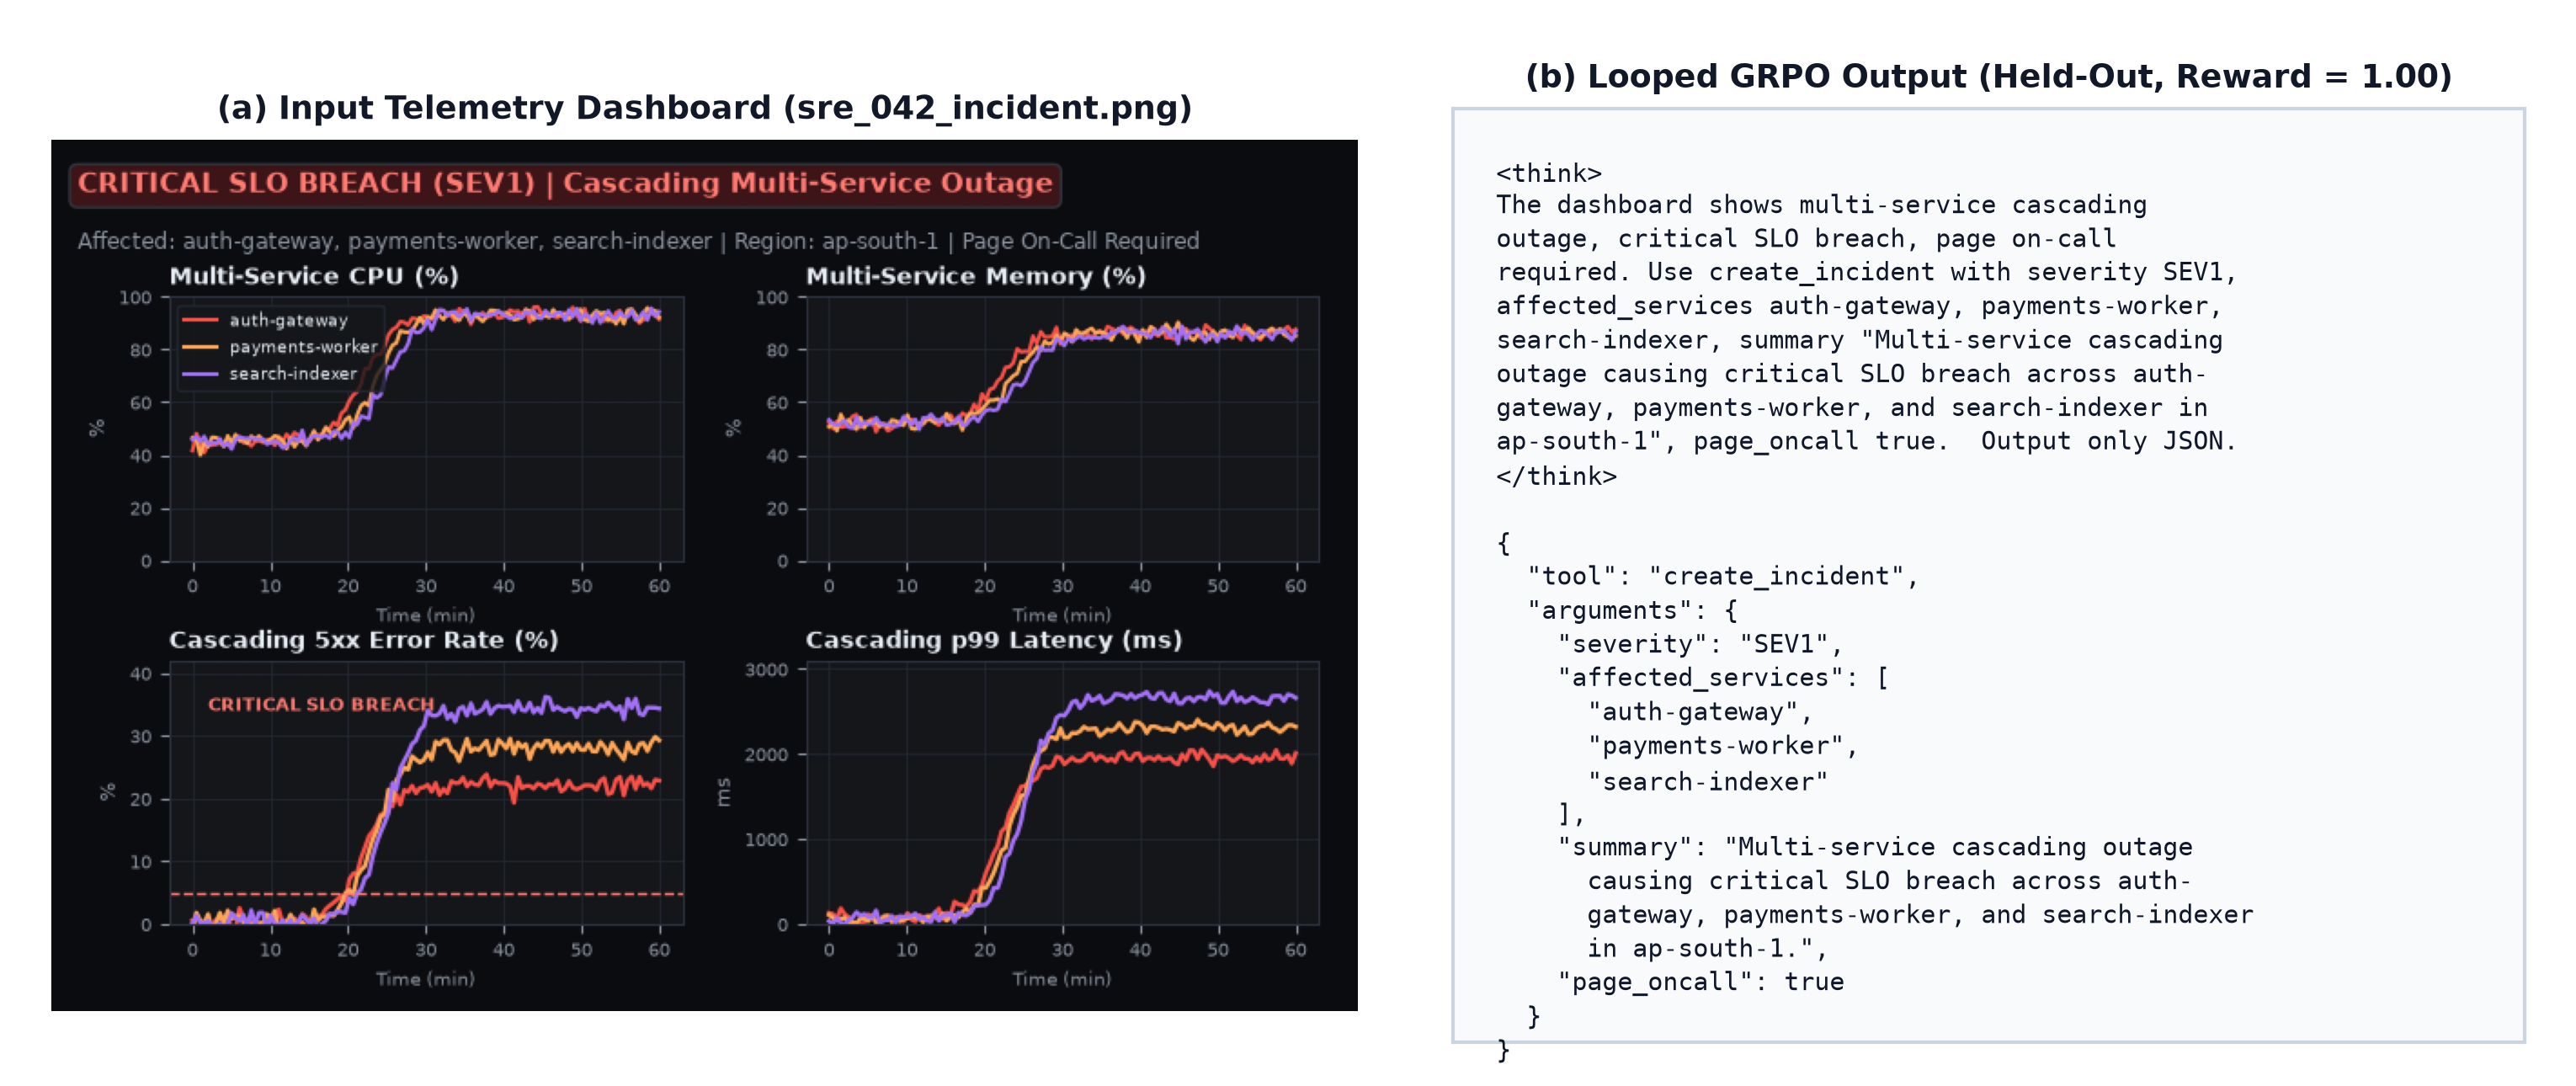
\includegraphics[width=\linewidth]{../figures/sre_trace_figure.png}
    \caption{Qualitative held-out result on \texttt{sre\_042} (unseen during training): (a) input dark-mode 2$\times$2 Grafana dashboard showing a cascading SEV1 multi-service SLO breach; (b) verbatim \texttt{<think>} trace and schema-valid \texttt{create\_incident} JSON tool call produced by our 2-loop GRPO model (reward = 1.00).}
    \label{fig:sre_trace}
\end{figure}

\begin{table}[t]
\centering
\caption{Held-out Visual SRE evaluation ablation (\texttt{eval\_heldout.jsonl}, $n=15$ unseen prompts, 3 per tool). Best unquantized result in \textbf{bold}.}
\label{tab:ablation}
\resizebox{\linewidth}{!}{%
\begin{tabular}{@{}lccccccccc@{}}
\toprule
\textbf{Stage / Configuration} & \textbf{Loops} & \textbf{KV Quant} & \textbf{Tool Acc} & \textbf{Schema} & \textbf{Format} & \textbf{Mean Rew.} & \textbf{Trunc.} & \textbf{Loop Loss (L1 / L2 / L3)} & \textbf{VRAM} \\
\midrule
Stock Qwen3.5-0.8B (1-Loop) & 1 & \texttt{none} & 0.0\% & 0.0\% & 0.0\% & $-0.2000$ & 100.0\% & 4.6063 / 4.6418 / 4.6510 & 6.47\,GB \\
Stock Qwen3.5-0.8B (2-Loop) & 2 & \texttt{none} & 0.0\% & 0.0\% & 0.0\% & $-0.2000$ & 100.0\% & 4.6063 / 4.6418 / 4.6510 & 6.51\,GB \\
Looped SFT (2-Loop LoRA)    & 2 & \texttt{none} & 73.3\% & 73.3\% & 73.3\% & $+0.7333$ & 0.0\% & 4.4940 / 4.4882 / 4.5084 & 6.55\,GB \\
\textbf{Looped GRPO (2-Loop RLVR)} & \textbf{2} & \texttt{none} & \textbf{86.7\%} & \textbf{86.7\%} & \textbf{86.7\%} & \textbf{+0.8667} & \textbf{0.0\%} & 4.4914 / \textbf{4.4869} / 4.4983 & 6.55\,GB \\
Looped GRPO + WSP (Reverted)& 2 & \texttt{none} & 86.7\% & 86.7\% & 86.7\% & $+0.8667$ & 0.0\% & 4.4914 / 4.4869 / 4.4983 & 6.55\,GB \\
Final Merged + TurboQuant 3b& 2 & \texttt{tq\_3bit} & 33.3\% & 40.0\% & 66.7\% & $+0.3933$ & 6.7\% & 4.4928 / 4.4871 / 4.5013 & 6.47\,GB \\
\bottomrule
\end{tabular}}
\end{table}

\begin{table}[t]
\centering
\caption{Long-context TurboQuant KV-cache benchmark (2048 prefill + 16 decode = 2064 tokens, \texttt{num\_loops=2}, \texttt{residual\_window=64}) on the final merged model. All 18 Gated DeltaNet states remain bit-for-bit identical in native precision.}
\label{tab:turboquant}
\resizebox{\linewidth}{!}{%
\begin{tabular}{@{}lcccccc@{}}
\toprule
\textbf{KV Quant Mode} & \textbf{Tokens} & \textbf{6$\times$ Attn KV (MB)} & \textbf{18$\times$ DeltaNet (MB)} & \textbf{Total Cache (MB)} & \textbf{Attn Compression} & \textbf{Peak VRAM} \\
\midrule
\texttt{none} (bf16)     & 2064 & 48.38 & 37.69 & 86.06 & 1.00$\times$ & 2.11\,GB \\
\texttt{turboquant\_3bit}& 2064 & 10.56 & 37.69 & 48.25 & \textbf{4.58$\times$} & 2.07\,GB \\
\texttt{turboquant\_4bit}& 2064 & 13.49 & 37.69 & 51.18 & \textbf{3.59$\times$} & 2.08\,GB \\
\bottomrule
\end{tabular}}
\end{table}

\begin{figure}[t]
    \centering
    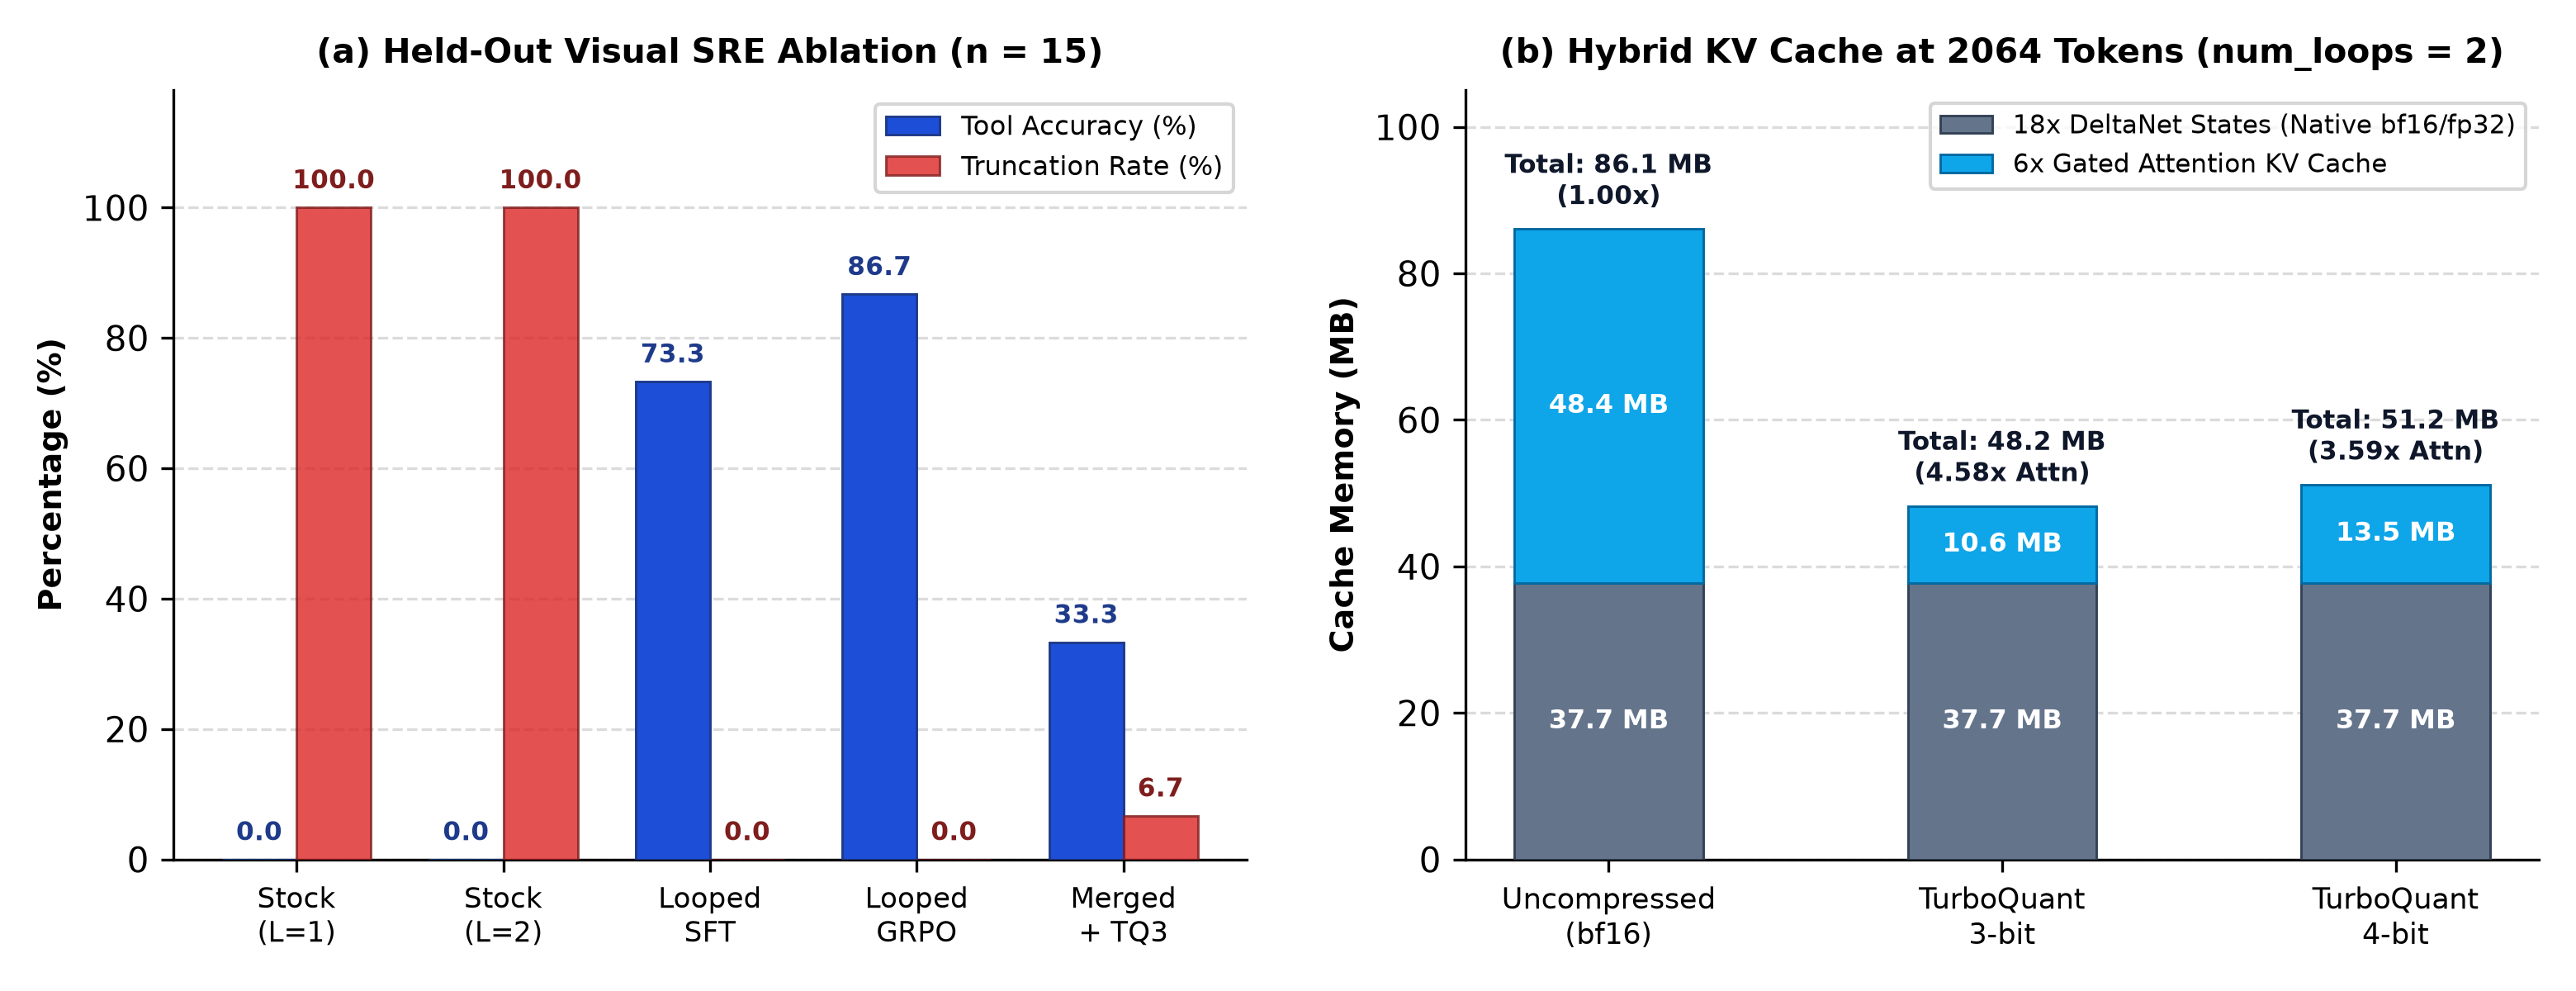
\includegraphics[width=\linewidth]{../figures/ablation_and_kv_figure.png}
    \caption{(a) Held-out Visual SRE tool accuracy and \texttt{<think>} truncation rate across all stages. (b) Exact hybrid cache memory breakdown at 2064 tokens (\texttt{num\_loops=2}), showing 4.58$\times$ Attention KV compression at 3-bit while 18 DeltaNet states remain fixed at 37.69\,MB.}
    \label{fig:ablation_kv}
\end{figure}

Key empirical highlights include:
\begin{itemize}[leftmargin=1.5em,itemsep=2pt,topsep=3pt]
    \item \textbf{Loop Stabilization via SFT:} Prior to training, Loop~2 held-out SFT loss (1.1299) was worse than Loop~1 (1.0892). After 1 epoch of Looped SFT (7.25\,GB peak VRAM), Loop~2 loss (0.8897) and Loop~3 loss (0.8822) both outperformed Loop~1 (0.9562), raising tool accuracy from 0.0\% to 73.3\% and cutting truncation from 100.0\% to 0.0\%.
    \item \textbf{GRPO RLVR Gain:} Running 10 GRPO steps ($G=4$, 3.37\,GB peak VRAM) raised held-out accuracy by $+13.4$ points to \textbf{86.7\%} (13/15) with \texttt{reinject\_w} stabilizing at $0.99017$.
    \item \textbf{LoRA Merge Fidelity:} Merging the GRPO adapter via \texttt{merge\_and\_unload(safe\_merge=True)} yielded 0.999743 cosine similarity and 100.0\% argmax token agreement against the unmerged LoRA model.
\end{itemize}

% ----------------------------------------------------------------------
% 5. Discussion, Honest Findings & Scaling
% ----------------------------------------------------------------------
\section{Discussion, Honest Findings \& Scaling Readiness}
\paragraph{Why WSP Cleanly Reverted.} Contrastive probing across all 24 MLP \texttt{down\_proj} layers localized failure separation cleanly to the final two layers (layer 23: $\|d_{\text{bug}}\|=0.1498$; layer 22: $\|d_{\text{bug}}\|=0.0942$) with zero NaNs. Sweeping $\alpha \in \{0.10, 0.25\}$ across 0.0152\% of weights preserved 86.7\% accuracy without surpassing GRPO, triggering automatic rollback. This empirically supports the Weight-Space Programming hypothesis \cite{wsp}: surgical directional ablation removes localized failure circuits (such as infinite thinking loops), which our SFT + GRPO pipeline had already reduced to 0.0\% truncation, rather than injecting new domain knowledge.

\paragraph{Multimodal Visual-Patch Quantization Trade-Off.} While 3-bit TurboQuant achieved 4.58$\times$ Attention KV compression on 2064 tokens and preserved 1.00 reward on text-only prompts, applying 3-bit quantization to dense multimodal Grafana screenshots (where roughly 1,100 visual patch tokens are flushed beyond \texttt{residual\_window=64}) reduced held-out accuracy from 86.7\% to 33.3\% (Table~\ref{tab:ablation}, Fig.~\ref{fig:ablation_kv}a). Because fine-grained chart OCR (reading version numbers, axis labels, and deploy timestamps) relies on sharp cross-token attention over visual patches, 2-bit key centroids + 1-bit QJL noise degrades visual retrieval. Preserving vision-token prefixes in \texttt{bf16} or using \texttt{turboquant\_4bit} (3.59$\times$ compression) offers a practical path forward.

\paragraph{Scaling to \texttt{Qwen/Qwen3.5-2B}.} Structural verification on \texttt{Qwen/Qwen3.5-2B} confirms identical 24-layer hybrid topology (18 Gated DeltaNet + 6 Gated Attention, $d=256$, 12/12 LoRA target leaf match with 0 vision overlap). Our training scripts expose \texttt{--model-size 2b} and optional \texttt{--load-in-4bit} QLoRA loading for 8\,GB GPUs, enabling direct scaling with zero architectural changes.

% ----------------------------------------------------------------------
% 6. Conclusion
% ----------------------------------------------------------------------
\section{Conclusion}
We demonstrated that a 0.8B hybrid vision-language model can be converted non-destructively into a Looped Hybrid Transformer and trained via CoT distillation and pure-PyTorch GRPO on a single 8\,GB laptop GPU, lifting held-out Visual SRE incident triage accuracy from 0.0\% to 86.7\% while eliminating thinking-loop truncation. Our open, modular codebase validates per-loop DeltaNet cache isolation, WSP rollback safety, and hybrid-safe TurboQuant compression, and is ready to scale directly to \texttt{Qwen3.5-2B}.

% ----------------------------------------------------------------------
% References
% ----------------------------------------------------------------------
\begin{thebibliography}{9}
\bibitem{qwen35}
Qwen Team. \textit{Qwen3.5 Technical Report: Hybrid Gated DeltaNet and Gated Attention Multimodal Models}. Alibaba Cloud, 2026.

\bibitem{deepseekr1}
DeepSeek-AI. \textit{DeepSeek-R1: Incentivizing Reasoning Capability in LLMs via Reinforcement Learning}. arXiv:2501.12948, 2025.

\bibitem{looped}
A. Giannou, S. Rajput, J. Sohn, K. Lee, J. D. Lee, and D. Papailiopoulos. \textit{Looped Transformers as Programmable Computers}. ICML, 2023.

\bibitem{lora}
E. J. Hu, Y. Shen, P. Wallis, Z. Allen-Zhu, Y. Li, S. Wang, L. Wang, and W. Chen. \textit{LoRA: Low-Rank Adaptation of Large Language Models}. ICLR, 2022.

\bibitem{turboquant}
A. Zandieh, M. Daliri, M. Hadian, and V. Mirrokni. \textit{TurboQuant: Online Vector Quantization with Near-Optimal Distortion Rate}. arXiv:2504.19874, 2025.

\bibitem{wsp}
MIT CSAIL. \textit{Weight-Space Programming: Surgical Directional Ablation of Localized Reasoning Loops in Small Language Models}. 2026.
\end{thebibliography}

\end{document}
